\documentclass[11pt,a4paper]{report}
\usepackage{tikz}
\usepackage[round]{natbib}
\title{Adding a spatial element to Outbreaker}
\begin{document}
\maketitle
\chapter*{Statement of Originality}
\thispagestyle{empty}
\noindent I certify that this thesis, and the research to which it refers, are the product of my own work, conducted during the current year of the MRes in Biomedical Research at Imperial College London. Any ideas or quotations from the work of other people, published or otherwise, or from my own previous work are fully acknowledged in accordance with the standard referencing practices of the discipline. The Outbreaker model referenced in this thesis is the work of Thibaut Jombart, Anne Cori, Xavier Didelot, Simon Cauchemez, Christophe Fraser and Neil Ferguson at the Department of Infectious Disease Epidemiology at Imperial College London.
\newpage

\chapter*{Abstract}
\thispagestyle{empty}
This is where my abstract goes
\newpage

\chapter*{Acknowledgements}
\thispagestyle{empty}
This is where my acknowledgements go
\newpage

\tableofcontents
\pagestyle{plain}
\newpage

\chapter*{Abbreviations}
\thispagestyle{empty}
This is where my abbreviations go
MCMC - Markov chain Monte Carlo
\newpage


\chapter{Introduction}
In certain outbreak scenarios it may be possible to separate the cases of infection into two or more distinct groups, the groups could be defined by what ward a patient is on in a hospital, what class a child is in at school or perhaps whether a case is a child or an adult. An interesting question in this scenario might be whether individuals in the same group are more likely to infect each other and less likely to infect individuals in the other group. Previous work which has sought to estimate transmission rates between different groups within a population has involved using large epidemiological datasets to fit a different compartmental model for each group, or the creation of bespoke models for specific outbreak scenarios. Crucially these approaches seek to estimate transmission rates between groups in isolation from other epidemiological properties; this approach relegates the study of the spatial structure of an outbreak to an afterthought, to be performed after more pragmatic epidemiological analyses have been undertaken.

In this paper we will add a spatial framework to an existing general Bayesian model (and corresponding R package Outbreaker) for predicting transmission routes of a pathogen during an outbreak. In the package, epidemiological and genetic data collected from outbreaks is used to derive samples from the posterior distribution of transmission trees. We will show how this method can be extended to include further data about the spatial structure of the population and see how well we can estimate parameters representing transmission rates between different groups. Additionally, this spatial data may also serve to improve the quality of the model output in situations where genetic data is not present; in the past genetic data has been shown to play an important role in placing constraints on potential transmission trees, making the job of finding the most likely transmission trees easier than with epidemiological data alone. By introducing group structure as part of an effective existing model it is hoped that this will allow the study of the spatial structure of the population during an outbreak to begin sooner, as well as inviting in any wider benefits that introducing this spatial framework may bring to other areas of the model.
\section{Aims}
The aim of this project is to see if information about the spatial structure of a population can be added to the Outbreaker model of \citet{outbrkr}, to estimate information about the rates of transmission between different groups or to further improve the process of deriving transmission tree samples from the posterior distribution using outbreak data. By adding this framework we will introduce parameters that will estimate these group transmission rates. In this first section we go through the previous body of work which led up to the development of the Outbreaker model before introducing the modelling techniques which are utilised in the Outbreaker model.


\section{A Brief History}
The Outbreaker package uses a Markov chain Monte Carlo process to try and sample from the posterior probability distribution of various parameters and pieces of augmented data. Specifically, it uses DNA sequence data and case data collected from an outbreak along with a generation time distribution and a time-to-collection distribution to infer the immediate ancestor of each case. These likely ancestors can be combined into a transmission tree, and if we are fairly confident in the truth of our assembled transmission tree then we can infer further properties about the outbreak from it. These properties include the rate of mutation of nucleotides in the DNA sequence of the pathogen and the effective reproduction numbers of individuals through time (which has important properties concerning the potential of an outbreak to become an epidemic [CITATION HERE Christophe's review paper?]).

The Outbreaker model builds upon previous methods that use a similar process of assigning a likelihood value to transmission trees (out of potentially thousands of tree configurations) and then searching for the tree with the maximum likelihood value or using the likelihood of a tree to sample from the posterior distribution over all possible trees given the data we have collected. The earliest implementation of this approach was \citet{Haydon03}, who proposed a likelihood function for transmission trees which might define the spread of foot-and-mouth disease between farms in the UK. Their likelihood function for each transmission event is a product of two independent terms. The first term gives a likelihood value based upon whether the timings of the infection between two farms match well. \citet{Haydon03} assigned a value based upon how well the period during which farm A was infectious overlaps with the predicted time period during which farm B was infected. The better these time periods overlap, the more likely this transmission event was. The second term gives a likelihood value based on how far apart the two farms are, seeing as animals on different farms do not freely mix (especially during an outbreak) then there is only the possibility of an aerial infection, this is more plausible the closer the two farms are. For each tree they considered the likelihood of all of the separate events in the tree and came to an overall likelihood for the tree. Finally, \citet{Haydon03} proposed an algorithm which would work towards finding the transmission tree with the highest overall likelihood.

As genetic sequencing became faster and cheaper [IS THIS ASSUMED KNOWLEDGE?], Cottam et al [REFERENCE PROCEEDINGS] could expand upon this previous model by including a genetic likelihood term. Now that most case data also included a DNA sequence of the pathogen then the DNA sequences could be compared to see if they could help figure out the immediate ancestor of each case. Infectious diseases mutate quickly, therefore mutations in the DNA sequences can occur between each generation of cases in an outbreak. We can compare the DNA sequences and produce a likelihood that one case is the ancestor of another case depending on how similar the two sampled DNA sequences are, the more similar two sequences are the more likely that one is an ancestor of the other. Cottam et al [ANOTHER CITATION] proceeded by selecting the transmission tree configurations which had the highest genetic likelihoods and then using the previous epidemiological likelihood (based on infection and collection times by \citet{Haydon03}) to choose 4 final trees which accounted for 95\% of the sum total of the likelihood for every possible tree. Further alterations to the model were made by \citet{Ypma13}, who combined the genetic and epidemiological likelihoods into a single term, therefore removing the assumption that the two likelihoods are independent. This is an important assumption to consider because more mutations will occur in a DNA sequence over longer periods of time so we expect that there will be some correlation between the generation times and the number of mutations that we find.

In the same year \citet{Morelli12} used a Markov Chain Monte Carlo (MCMC) approach to sample from the posterior distribution of transmission trees given the collected data. This technique begins with a tree and then moves the suspected ancestors of each case around according to certain probability rules to form a new tree. The likelihood of both of these trees are calculated and the new tree is accepted as a sample with a probability calculated from the ratio of the two likelihoods. The chain and the movement rules are constructed so that the probability of accepting a tree as a sample is equal to the posterior probability of the tree given the data. We can then look at the trees with the highest posterior probabilities or consider the posterior probability that one case is an ancestor of another.

The Outbreaker model is a combination of these approaches, it uses an MCMC approach with independent genetic and epidemiological likelihoods. It also allows for unsampled cases to occur between two cases and a more complex account of the DNA sequence mutations. Unlike the previous approaches it can also be generalised into a package for the programming language R [CITE R PROPERLY] which means it can be run on personal computers by people with less technical computing skills within a reasonable amount of time. To understand the Outbreaker model we must first look at MCMC methods in general and understand how we can use an MCMC method to sample from a specified distribution.

\section{Markov Chain Monte Carlo Processes}
Markov Chain Monte Carlo processes are a combination of two statistical tools, the easiest of the two is Monte Carlo methods. Monte Carlo methods aim to approximate values such as the expected value of a probability distribution by using a large number of samples from that distribution. To work out the expected value of a probability distribution analytically we would integrate over every possible value in the distribution multiplied by the probability of it occurring:
\[ E(X) = \int_{-\infty}^{\infty} x \cdot p(x) dx \]
Using Monte Carlo methods we would approximate this integration by sampling from the probability distribution thousands of times and taking the mean average of the results:
\[ E(X) \approx \frac{1}{N}\sum_{i=1}^{N} X_i \] 
Put simply, Monte Carlo methods are a way of approximating values of interest given lots of the right samples.

Markov Chains play the role of providing these samples, a Markov Chain is a chain of subsequent states where the next state in the chain is decided by probabilities which are determined only by the current state. A simple discrete Markov Chain may have 3 states called A, B and C, if we are currently in state A then whatever state we move to next only depends on the probability of moving from state A to states B or C (or back to A). If I then move to state B, the fact that I was just previously in state A does not play a role in my decision making about what state I will go to next. If we run certain Markov Chains for long periods of time we will find that they settle into a stationary distribution which determines what the probability of the chain being in each state at any time is. If we have a stationary distribution of interest, such as $p(X=A)=p(X=B)=p(X=C)=\frac{1}{3}$ then we can devise a Markov Chain that will have states A, B and C that has this distribution as its stationary distribution. We can run this Markov chain for a while until it converges upon its stationary distribution and use the values in the Markov Chain as samples from this distribution of interest. MCMC methods combine the two methods by sampling from a Markov chain and then using these samples to estimate properties of their distribution.

We can use the Metropolis-Hastings algorithm to easily find Markov Chains that have a specified stationary distribution, therefore our stationary distribution could be very complex and we could still use a fairly simple Markov Chain to sample from it. We can then use these stationary distribution samples in our Monte Carlo methods to make approximations about the distribution. Metropolis-Hastings can also be used in a Bayesian setting by specifying the stationary distribution as a posterior distribution of interest. This means that instead of having to find a posterior distribution analytically we can instead use an MCMC process to sample from it and then make inferences about the distribution from our samples. This is what the Outbreaker model does in the specific context of finding the posterior distribution of transmission trees with given outbreak data. The posterior distribution that the Outbreaker model tries to sample from is complex, yet we can use the relatively straightforward Metropolis-Hastings algorithm to construct a Markov Chain with a stationary distribution equal to our posterior distribution.


\section{The Metropolis-Hastings Algorithm}
\citet{Voss14} describes how we can use the Metropolis-Hastings algorithm to sample from our target density $\pi$ as follows:
\begin{itemize}
\item Start with a value $X_0$ that is from the target density, thus $\pi(X) > 0$.
\item We then need a transition density $p(x,y)$ where $p(x, \cdot)$ is the probability density of the next possible states of the Markov chain given that the previous state was $x$. We then sample a value $X_1$ from the distribution $p(X_0,\cdot)$.
\item We then calculate 
\[ \alpha(X_0,X_1) = min\left(\frac{\pi(X_1)p(X_1,X_0)}{\pi(X_0)p(X_0,X_1)},1\right) \]
\item We then generate a random variable $U_1 \sim U[0,1]$, if $\alpha(X_0,X_1) > U_1$ then we accept $X_1$ as a sample from $\pi$. If not then we set $X_1 \leftarrow X_0$ and accept this as a sample.
\item We repeat this process for thousands of iterations, saving all of the accepted values in a chain. These values are samples from our target density $\pi$.
\end{itemize}
The need to find the values $\pi(X)$ presents a problem because it requires that we know (or can at least find probability values from) the target distribution which we are trying to sample from and this might not be the case. We can get around this when looking for posterior densities by substituting in the likelihood function which is usually easier to calculate. If our target density is a posterior density of the form $\pi(\theta | D)$ with parameter $\theta$ and observed data $D$ then we can write this as
\[ \pi(\theta | D) \propto \frac{\pi(D | \theta) \times \pi(\theta)}{\pi(D)} \]
Since $D$ represents fixed data, $\pi(D)$ is a constant and therefore cancels out in the equation for $\alpha(x,y)$ so we are left with
\[ \alpha(X_0,X_1) = min\left(\frac{\pi(D | X_0)\pi(X_0)p(X_1,X_0)}{\pi(D | X_1)\pi(X_1)p(X_0,X_1)}\right) \]
Therefore to use Metropolis Hastings to sample from a posterior distribution we only need to be able to construct the likelihood function and calculate values from the prior densities of our parameters.


\section{The Outbreaker MCMC Process}
Outbreaker uses the Metropolis-Hastings algorithm to sample from the posterior distribution of transmission trees when we have data on an outbreak. There is a transition density that moves around parameters such as the rate of DNA mutation and then accepts or reject the candidate parameter based on the genetic likelihood defined in the Outbreaker model. Additionally Outbreaker uses augmented data which are pieces of data that are moved around as if they were parameters and accepted or rejected. In the context of Outbreaker each case $i$ has an ancestor $\alpha_i$; a transition density is used to suggest a new candidate ancestor, the likelihood of this potential ancestry is calculated depending on how well the infection time, spatial and DNA sequence data fit together between the cases. We can now go on to to discuss how the new group structure data and group likelihood fit into the current Outbreaker model.


\chapter{Methods}
\section{Group Data and Parameters}
As previously mentioned, certain outbreak scenarios lend themselves to a model whereby the population is separated into distinct groups, people in these groups could have different levels of contact between members of their own group and members of other groups. This could potentially lead to different rates of transmission within and between different groups. One example of this could be groups of patients on different wards of a hospital, if someone on one ward falls ill it seems plausible that they are more likely to transmit this infection to another patient on their own ward rather than a patient on a different ward. If the outbreak spreads through several wards we could use our knowledge of what ward cases are on to assess the probability that one case infected another and help us construct a transmission tree. Another example could be to separate cases into groups based on their age, several studies have looked into how the probability of common cold transmission differs from child to child, child to adult, adult to child and adult to adult [CITE THE STUDIES PLZ].

We represent these differing rates of transmission between $l$ groups as parameters in an $l \times l$ transmission probability matrix where the element $p_{12}$ is the probability that a case's immediate ancestor is in group 2 given that the case is in group 1.
\[ \left( \begin{array}{cccc}
p_{11} & p_{12} & \cdots & p_{1l} \\
p_{21} & p_{22} & \cdots & p_{2l} \\
\vdots & \vdots & \vdots & \vdots \\
p_{l1} & p_{l2} & \cdots & p_{ll} \\
\end{array} \right) \] 

To introduce these parameters into the MCMC process we need to propose a transition density (also known as a "move") that will produce candidate transmission probabilities and a likelihood function that will be used to accept or reject candidate probabilities depending on how well they fit the data on what group each case is in.

\section{Group Likelihood}
The existing pseudo-likelihood function of the outbreaker model is composed of the product of the genetic and epidemiological likelihoods. We need to construct a group likelihood function to multiply onto the existing likelihood function, the group likelihood function will give us a likelihood value for the probabilities in our transmission matrix given the observed and augmented data. Some of the observed and augmented data will not play a role in determining how likely the transmission probabilities are, such as the genetic sequences and timings of each case. The data that will play a role are $\alpha_i$, the index of the ancestor of case $i$ (and their corresponding group) and $\kappa_i$, the number of generations between $i$ and $\alpha_i$.\\

To write the group likelihood we can think of the transmission event between case $i$ with group $g_i$ and its immediate ancestor $\alpha_i$ with group $g_{\alpha_{i}}$ as a Bernoulli trial with $P_{g_i g_{\alpha_{i}}}$ chance of succeeding. We know the group membership of each case and the current candidate ancestor $\alpha_i$, therefore the likelihood of a transmission event between $i$ and $\alpha_i$ for the candidate transmission rates matrix, denoted $L$, is given by:
\[ \Omega_i^3 = p(g_i = x | \alpha_i, \kappa_i, g_{\alpha_i}=y, L) \]
and the likelihood of a Bernoulli trial is the probability that the event takes place, which can be found by calculating the transmission probability matrix, so for this particular case the likelihood is:
\[ \Omega_i^3 = P_{xy} \]
In the Outbreaker model each transmission event is assumed to be independent of other events, therefore the group likelihood for a whole transmission tree is the product of all of the individual likelihoods for each transmission event (or the sum of the group log likelihoods).
\[ \Omega^3 = \prod_i{\Omega_i^3} = \prod_i{P_{g_i g_{\alpha_i}}} \]
This likelihood term is multiplied onto the existing likelihood term to give an overall likelihood for a case: $\Omega_i^1 \times \Omega_i^2 \times \Omega_i^3$. This assumes that the group, epidemiological and genetic likelihoods are all independent. This assumption simplifies the likelihood term but in real outbreak data we would expect to see some correlation between the likelihood terms. For example, if transmission rates really were higher within a group than between other groups we might expect that observed DNA sequences are generally more similar between cases in the same group because mutations that occur between two cases in the same group are more likely to stay within that group, therefore distinguishing the DNA sequences from these cases from those belonging to other groups. Having defined our group likelihood term we must now decide upon the way in which the Metropolis-Hastings algorithm will move the parameters in the transmission rate matrix to produce new candidate rates.


\section{Transmission Rate Matrix Move}
We implemented a move for the transmission probabilities matrix in the MCMC algorithm which proposes new probabilities for each row of the matrix at a time, $l$ candidate probabilities are sampled from the Dirichlet distribution with concentration parameters equal to the old probability values in the chain multiplied by a constant value. This constant value is increased or decreased to keep the rate of acceptance of the move between 25 and 50\% for each row. The Dirichlet distribution is not symmetrical so we need to introduce a correction factor to account for the fact that in the transition density $p(x,y) \neq p(y,x)$. The prior distribution for each row is a symmetric Dirichlet distribution where all concentration parameters are equal and multiplied by a constant provided by the user. The multiplication constant reflects how confident the user is that the probabilities in the matrix are equal, larger values reflect a belief that the transmission probabilities are not equal between groups. This gives the following process for updating an element in the transmission rates matrix, it is the standard Metropolis-Hastings algorithm except we have taken the logarithm of values to preserve accuracy during computation:
\begin{itemize}
\item For row $i$ we take the current probabilities, ${\bf p}_{n} =  \{p_{i1},p_{i2}, \cdots,p_{il}\}$ and sample candidate probabilities: ${\bf p}_{n+1} \sim Dir(m{\bf p})$ where $m$ is the multiplying constant.
\item Calculate the log ratio: $ LR = \log(\Omega_3({\bf p}_{n+1})) - \log(\Omega_3({\bf p}_{n}))$
\item Add the correction factor for the Dirichlet distribution, if we define $Dir({\bf \alpha,x})$ as the probability distribution function of the Dirichlet distribution with concentration parameters ${\bf \alpha}$ evaluated at the values ${\bf x}$ then the correction factor is given by: 
\[ LR + \log(Dir({\bf p}_{n+1},{\bf p}_{n})) - \log(Dir({\bf p}_{n},{\bf p}_{n+1})) \]
\item Add the values of the priors for the old and candidate rates, with the user specified constant $c$ and concentration parameter ${\bf \alpha}$ with elements $\alpha_i$ all equal this is given by: 
\[ LR + \log(Dir({\bf \alpha},{\bf p}_{n+1})) - \log(Dir({\bf \alpha},{\bf p}_{n}))\]
\item If $LR > 0$, we accept ${\bf p}_{n+1}$ as a sample.
\item If $LR < 0$ then we generate a random uniform number, $U$, then if $\log(U) \leq LR$ then we accept ${\bf p}_{n+1}$ as a sample. Otherwise we reject ${\bf p}_{n+1}$ and ${\bf p}_{n+1} \leftarrow {\bf p}_{n}$.
\end{itemize}
The result of this process is a number of samples of the group transmission rate parameters from the posterior distribution, we can now go on to discuss how we can analyse this output and how we can produce data to test the extended model.




\section{Simulating Outbreaks With Group Structure}
To test the new spatial framework in Outbreaker, we need to be able to fit the model to data which was generated using a population that has groups which have varying tranmission rates between them.
The Outbreaker package has its own outbreak simulation procedure, {\tt simOutbreak}, which we can extend to generate outbreak data that has the desired spatial structure. We can modify the formula which chooses the infector of an infected individual (in the program code this is implemented by first choosing the ancestors and then choosing who has been infected by them), currently the individual is chosen by sampling from a multinomial distribution with probabilities:
\[ \frac{w(t-t_i)}{\sum_i{w(t-t_i)}} \]
where $w$ is the generation time distribution. We can incorporate the probability of transmission within and between members of different groups into these probabilities by supplying a transmission probability matrix. If we continue with the notation $g_{i}$ as the group of case $i$ and $g_{\alpha_{i}}$ as the group of the immediate ancestor of case $i$ then we can introduce the group transmission probabilities into the multinomial distribution as follows:
\[ \frac{P_{g_{i}g_{\alpha_{i}}} \cdot w(t-t_i)}{\sum_i{P_{g_{i}g_{\alpha_{i}}} \cdot w(t-t_i)}}\]

At the start of the outbreak we would have $n$ individuals, $n_1$ of whom are in group 1, $n_2$ of whom are in group 2 and so on up to group $l$. We can then specify the exact numbers in each group ,perhaps indirectly through proportions of the population in each group, when the simulation begins. We would also specify the $l \times l$ matrix of transmission probabilities which would be the true, unknown parameters in our model tests. Then the procedure takes place just as before but now new cases have different probabilities of being infected by the existing cases depending on the within and between group transmission probabilities. We can then modify the output of {\tt simOutbreak} to colour the nodes of the transmission tree depending on group so it is easy to see how the outbreak has moved around the group structure. We would also need to come up with a rule for the group membership of imported cases - they could either be assigned to the existing groups at some specified frequency or marked as group unknown, which would bring up further questions about how to treat these cases in terms of transmission probabilities. In some situations such as hospital wards it might be sensible to take the first approach, our groups might be in one large ward and one small ward so we would expect imported cases to have joined one of the wards and although their ancestors are not present in our transmission tree we expect them to inherit the transmission dynamics of their group once they join one. For the second scenario we would have to decide what would be a sensible transmission probability between each group and a case where the group is unknown, we might assign a "baseline" transmission probability that we use for any cases where one or both of the groups are unknown during a transmission event. This is a better approach if our groups are set within a larger community that has some probability of transmission between the members (this is equivalent to assigning all imported cases to an extra group with equal within and between group transmission). Another benefit of this second approach is that it also provides a way of dealing with cases where group membership data is missing.

Having implemented this method in simOutbreak, the user can now pass a matrix to the simOutbreak function giving the true values of the transmission probabilities within and between groups, the user must also specify the number of individuals within each group. The number of individuals in each of the groups must sum to the overall number of individuals in the simulation, individuals are then assigned to groups randomly. Imported cases are assigned a group based on the relative sizes of the groups defined by the user. Users can now also colour nodes on the plotted transmission trees by their group membership, this allows us to see how the transmission tree is affected by different group sizes and transmission probabilities. For example, the tree below was created and coloured using three groups with the transmission probability matrix
\[ \left( \begin{array}{ccc}
0 & 1 & 0 \\
0 & 0 & 1 \\
1 & 0 & 0 \\
\end{array} \right) \]
\begin{center}
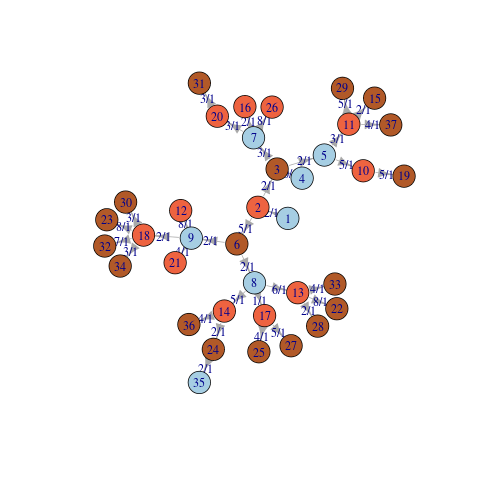
\includegraphics[width=180px]{treexample.png}
\end{center}
We can now go on to generate some data to see how the method performs on generated data and data from a real outbreak with spatial structure.

\chapter{Results}
\section{Testing Procedures}
We tested the extended method on simulated data with a spatial structure generated by the new simOutbreak function. The efficacy of outbreaker for reconstructing transmission trees in different situations has been researched before in [cite outbreaker paper] so we kept our focus on results relating to the new spatial framework. There were two principle aims of our testing: the first was to see how well outbreaker estimated the transmission probabilities between groups for datasets where the correct ancestries are already well determined by the DNA sequence data; the second was to see if providing the model with strong and correct priors for the group transmission probabilities helped infer correct ancestries for datasets which have a strong spatial signal and where DNA sequence data is not as advantageous as usual. 

\section{Estimating Transmission Probabilities}

For the first set of simulations we required datasets where outbreaker could already infer the majority of correct ancestries, we could then give outbreaker the spatial data and an uninformative prior and see how well the posterior distributions of the transmission probability parameters capture the spatial dynamics of the data.



We used an imagined scenario of collecting outbreak data from districts within a city in West Africa during the 2014 Ebola Virus Disease (EVD) outbreak. The study of the outbreak led the \citet{Ebola14} to hypothesise that the spread of EVD was in part due to a large amount of population movement between cities in bordering countries. We aimed to recreate this migration led transmission on a smaller scale between districts in a city. We created datasets where infected individuals are divided into groups based upon their district of residence and the probabilities of transmission between groups is dependent on the amount people travelling between the two districts. If many people commute between districts A and B regularly then it is more likely that an individual unknowingly infected with EVD will travel from district A to district B (or vice versa) and transmit EVD to the people who live there during their trip. To make the scenario as realistic as possible  we used the estimated epidemiological properties of EVD estimated during the recent analysis by \citet{Ebola14}.

\begin{tabular}{| c | c | c |}
Parameter & Value & Source \\
Serial Interval & Gamma distribution with mean = 13.5, s.d. = 9.2 & \citet{Ebola14} \\
$R0$ & 1.9 & \citet{Ebola14} \\
Mutation Rates & Substitution rate (transversions) per site per day =  5.479452e-06 & \citet{Gire14} \\

\end{tabular}

We created NUMBER datasets using these parameters and ran several instances of outbreaker on each dataset. For each dataset outbreaker was run using DNA and spatial data, DNA data only, spatial data only and neither of the two types of data (leaving only dates of symptom onset and the epidemiological likelihood of the model). We then analysed the proportion of correct ancestries inferred on each run for each dataset to check that the transmission tree was adequately inferred using DNA sequence data alone and that the outbreaker model including the spatial framework was behaving correctly. The violin plot below shows the proportions of correct ancestries by each run over all of the simulated datasets. 
\\
VIOLIN PLOT GOES HERE
\\
In line with previous results from \citet{outbrkr}, outbreaker infers a much higher proportion of correct ancestries when DNA sequence data is included. Comparing runs with and without spatial data also shows that the outbreaker model including the spatial framework performs as well as, if not very slightly better, than the original outbreaker model. We also checked the convergence of the model likelihood including the spatial likelihood for several datasets to ascertain that the model with the spatial data was mixing well and converged upon a posterior distribution suitably, an example of one of these MCMC traces is shown below. The outbreaker runs including spatial data had uninformative priors that suggested that all group transmission probabilities are equal. If all group transmission is equal we can conclude that dividing the cases into these groups does not provide us with any new information about the spatial dynamics of the outbreak. 
\\
TRACE GOES HERE
\\
Once we were satisfied that the extended outbreaker model was running properly we could then begin to scrutinise the posterior density samples for the transmission probability parameters. Each simulation was generated using the same transmission probability matrix but the number of cases varied so the simulations as a whole should give a good idea of how well the parameters are inferred in a variety of situations. Our first step in evaluating the posterior samples for each run was to see in the true parameter value (used to generate the dataset) fell inside the 95\% equal-tails interval, we then counted how many times this occurred for each parameter over all of the simulations to give us a rough idea of how often outbreaker infers a posterior distribution with a reasonable probability of giving the true parameter value.
\\
SOME KIND OF PLOT OR MATRIX SHOWING RESULTS HERE
\\
We also calculated the posterior sample median for each transmission probability parameter and produced a BOXPLOT/VIOLIN PLOT to describe where the sample medians fell over all of the simulations.
\\
BOX/VIOLIN PLOT HERE
\\



\section{Inferring Correct Ancestries}
We also hoped to show that the spatial likelihood could help to infer correct ancestries in situations where the genetic and epidemiological likelihoods were not so effective. These situations are characterised by an outbreak where there not much mutation occurring in the DNA sequences between cases and a fairly long generation time. In these situations the original outbreaker model without spatial data struggles to infer the correct ancestor for two reasons. The genetic likelihood cannot narrow down the ancestor because there are few mutations between cases so most previous cases will have very similar genetic likelihoods. Secondly, the epidemiological likelihood struggles because the fairly long generation time means that for a newly infected case we have to look quite far back into the past for potential ancestors, this will bring up many candidate ancestors and we have no other way to determine who the correct ancestor is likely to be. In the transmission tree below, if there are not many mutations between cases, we would have trouble inferring an ancestor out of cases 1 to 5.
\\
\begin{center}
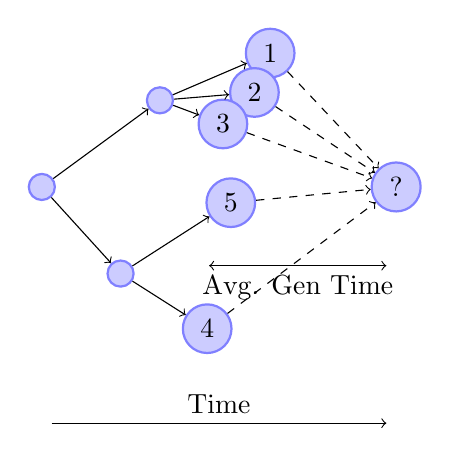
\begin{tikzpicture}
	\node at (0,0) (1){};
	\node at (4.5,0) (2){};
	\node at (0,3) [circle, draw=blue!50, fill=blue!20, thick] (c1) {};
	\node at (1.5,4.1) [circle, draw=blue!50, fill=blue!20, thick] (c2) {};
	\node at (1,1.9) [circle, draw=blue!50, fill=blue!20, thick] (c3) {};
	\node at (2.9,4.7) [circle, draw=blue!50, fill=blue!20, thick] (c4) {1};
	\node at (2.7,4.2) [circle, draw=blue!50, fill=blue!20, thick] (c5) {2};
	\node at (2.3,3.8) [circle, draw=blue!50, fill=blue!20, thick] (c6) {3};	
	\node at (2.1,1.2) [circle, draw=blue!50, fill=blue!20, thick] (c7) {4};
	\node at (2.4,2.8) [circle, draw=blue!50, fill=blue!20, thick] (c8) {5};		
	\node at (4.5,3) [circle, draw=blue!50, fill=blue!20, thick] (c9) {?};
	\node at (2,2) (3) {};
	\node at (4.5,2) (4) {};
	
	\draw [<->] (3) -- (4) node[midway,below] {Avg. Gen Time};
	\draw [->] (1) -- (2) node[midway, above] {Time};
	\draw [->] (c1) -- (c2); 
	\draw [->] (c1) -- (c3);
	\draw [->] (c2) -- (c4); 
	\draw [->] (c2) -- (c5); 
	\draw [->] (c2) -- (c6);
	\draw [->] (c3) -- (c7); 
	\draw [->] (c3) -- (c8);
	\draw [->] (c4) -- (c9)[dashed]; 
	\draw [->] (c5) -- (c9)[dashed]; 
	\draw [->] (c6) -- (c9)[dashed];
	\draw [->] (c7) -- (c9)[dashed]; 
	\draw [->] (c8) -- (c9)[dashed];
	
	
	
	 	 			 
\end{tikzpicture}
\end{center}	
The group likelihood can help in this situation if the cases are divided into groups and we have are confident of what the group transmission probabilities in the situation are. If we are sure that most transmission takes place within groups we could provide a prior that heavily promotes unequal transmission probabilities, this can give us another way of determining the most likely ancestor of a case when the genetic and epidemiological likelihoods are not useful.  An unequal transmission probability prior will reward candidate transmission probabilities that are unequal, this gives a transmission probability matrix with values that are more unequal (because there is a higher probability of accepting candidate probability values that are more unequal due to our specified prior). If the data has a true spatial structure where transmission happens overwhelmingly within groups this will be inferred quickly by the model because it is encouraged by the prior. Therefore when we go to assess the group likelihood of a particular ancestry, it will give a much higher likelihood value to two cases within the same group. Returning to the scenario from the previous paragraph, if the newly infected case belongs to group A and there are 5 candidate ancestors, one of whom belongs to group A, then the likelihood of the connection between the two cases from group A will be much higher and therefore outbreaker will infer this ancestry. Therefore if our prior knowledge that the transmission rates are very unequal is true then we will have biased outbreaker towards the correct ancestries based on their group membership. This is how the spatial structure of the data and a strong prior can help outbreaker infer correct ancestries in certain situations where the other data is not as useful. In the transmission tree below the nodes are coloured by group membership. If we are trying to guess an ancestor for the new case and we suspect that most transmission occurs within groups then we would guess node 5. If our prior knowledge is accurate then we are making a sensible guess because it would be most likely to have been node 5 that infected our new case. Adding in a spatial structure and prior knowledge has helped us infer the correct ancestor.
\begin{center}
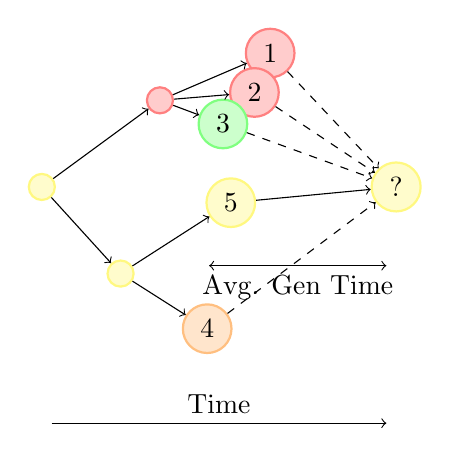
\begin{tikzpicture}
	\node at (0,0) (1){};
	\node at (4.5,0) (2){};
	\node at (0,3) [circle, draw=yellow!50, fill=yellow!20, thick] (c1) {};
	\node at (1.5,4.1) [circle, draw=red!50, fill=red!20, thick] (c2) {};
	\node at (1,1.9) [circle, draw=yellow!50, fill=yellow!20, thick] (c3) {};
	\node at (2.9,4.7) [circle, draw=red!50, fill=red!20, thick] (c4) {1};
	\node at (2.7,4.2) [circle, draw=red!50, fill=red!20, thick] (c5) {2};
	\node at (2.3,3.8) [circle, draw=green!50, fill=green!20, thick] (c6) {3};	
	\node at (2.1,1.2) [circle, draw=orange!50, fill=orange!20, thick] (c7) {4};
	\node at (2.4,2.8) [circle, draw=yellow!50, fill=yellow!20, thick] (c8) {5};		
	\node at (4.5,3) [circle, draw=yellow!50, fill=yellow!20, thick] (c9) {?};
	\node at (2,2) (3) {};
	\node at (4.5,2) (4) {};
	
	\draw [<->] (3) -- (4) node[midway,below] {Avg. Gen Time};
	\draw [->] (1) -- (2) node[midway, above] {Time};
	\draw [->] (c1) -- (c2); 
	\draw [->] (c1) -- (c3);
	\draw [->] (c2) -- (c4); 
	\draw [->] (c2) -- (c5); 
	\draw [->] (c2) -- (c6);
	\draw [->] (c3) -- (c7); 
	\draw [->] (c3) -- (c8);
	\draw [->] (c4) -- (c9)[dashed]; 
	\draw [->] (c5) -- (c9)[dashed]; 
	\draw [->] (c6) -- (c9)[dashed];
	\draw [->] (c7) -- (c9)[dashed]; 
	\draw [->] (c8) -- (c9);
	
	
	
	 	 			 
\end{tikzpicture}
\end{center}
To test this we created datasets that had small groups with 3-4 people in (households) and one larger group (the community), the true transmission probabilities were such that cases with a household had very high probabilities of infecting individuals in the same household, a much lower probability of infecting individuals in the community and an extremely low probability of infecting individuals in other households. Cases in the community had a reasonable probability of infecting others in the community and the rest of the probability was assigned equally to infected a member from each household. The aim of this was to try and create datasets where most transmission happened within households and infection spread from household to household via the community where the equal probability of moving to a new household modelled random mixing in a community setting. In these datasets there would be several new cases occurring in different households at the same time, if we take into account the household structure then we would assume that a new case in household A was infected by a previous case in household A. If we do not have any spatial framework in outbreaker then we have a collection of cases that happened around the same time with barely any differences in the DNA sequences between them. The transmission tree below is from such a dataset, the node colours represent the group that the case belongs to. The light blue nodes are members of the community, other colours are members of different households.
\begin{center}
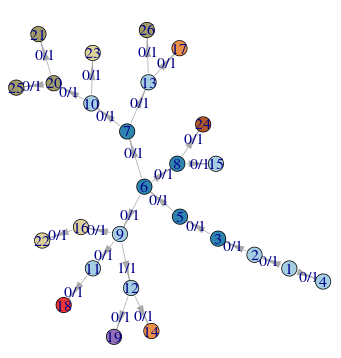
\includegraphics[scale=0.6]{ancestree.png}
\end{center}
As described, most transmission takes place between members of the same household and the infection mostly moves from household to household via the community. We ran two different instances of outbreaker on this dataset to see which one could infer the correct ancestries better, one run had no spatial data and the other had spatial data and priors that strongly favoured unequal transmission probabilities.







\section{Equine Flu Data}
To test the method on real outbreak data we used some of the dataset of the 2003 equine influenza outbreak in Newmarket provided with the R package OutbreakTools, the dataset contains pathogen DNA sequence data and sequence collection dates for 121 individuals in 25 different paddocks. We chose to define the group of each case to be their corresponding paddock number and took a subset of the data from the beginning of the outbreak (to keep group numbers small and the number of individuals in each group reasonable) and tried to reproduce the transmission tree inferred by [Joseph’s Equine Flu paper].



\chapter{Discussion}
\section{Discuss Results}
\section{Modelling Assumptions}
This way of modelling group structure makes some simplifying assumptions, it is important to recognise these assumptions and consider how they may effect the interpretation and usefulness of the model output. The first and main assumption is that the likelihood terms for the genetic, epidemiological and spatial data are independent, this would imply that we expect no correlation between the likelihoods for our data, yet we would actually expect there to be some correlation. We would expect cases which occur around a similar time to have a high epidemiological likelihood of transmission between each other, but this short time frame means that there has not been much time for the pathogen DNA sequences to diverge, therefore we would also see that some of these cases have similar pathogen DNA sequences and therefore a high genetic likelihood between them. As the Markov Chain approaches true transmission events we would see that the likelihoods rise and fall together, rather than being independent of each other. However, combining these likelihoods would be a very tricky process and would inevitably produce a more complex likelihood function - this has consequences in terms of computational effort when we attempt to compute the likelihood function for thousands of moves. It is also hard to gauge what sort of effect this assumption will have on the output of the model without computing a combined likelihood and comparing the results. One possibility is that having separate likelihoods which are correlated could inflate the overall likelihood value for a tree in places where the individual likelihoods are high. This could lead to a likelihood landscape with more drastic peaks and troughs, making it harder for the Markov Chain to jump between these areas of high likelihood.

A second, less worrying assumption is that transmission probabilities between groups remain constant over time. This assumption serves to constrain the situations in which this model would be appropriate, depending on whether the assumption would be violated. In most of the scenarios envisioned, such as an outbreak in a hospital ward, it is probably safe to assume that the transmission rate between groups stays fairly constant over the period of the outbreak. However, this does rule out the model being used to assess the effectiveness of an intervention on reducing the transmission rates between groups where all of the data comes from the same outbreak. Although data from two outbreaks that are similar in every other respect apart from the presence of an intervention strategy during one of the outbreaks could be used to compare the effectiveness of the intervention strategy at preventing between group transmissions.


\section{Modelling Limitations}
In this section I will discuss constraints placed upon the model by adding the group structure framework and vice versa. The new parameters in the model cannot be considered too helpful if they unduly restrict other parts of the model. In this case the significant restraint placed on the rest of the model by the group transmission parameters is that we must assume that there are no unsampled cases between infected individuals, thus limiting the situations in which we can use the extended model to those where we can be sure that we have collected data on every case in an outbreak. These sorts of outbreak would be relatively small and in places where data can easily be collected, thankfully the imagined scenario of different wards in a hospital matches this description.

When we are dealing with transmission between two cases where there are unsampled cases between them we do not know the group membership of the unsampled cases which causes problems when we come to assess the likelihood of this transmission event. For example if Rob is in red ward and Mary is in blue ward and we are considering the group likelihood of a transmission event between them with one unsampled generation, Alice say, then the group likelihood would be the product of two probabilities, that Rob gave the infection to Alice and then that Alice gave the infection to Mary. The problem is that we don't know what group Alice belongs to so we don't know what the relevant group transmission probabilities are.


\section{Not finished yet}
would sum the likelihoods that Rob infected Alice who then infected Mary for the case that Alice is a member of any possible group - in this case red or blue ward.\\
For small values of $\kappa$ we can easily calculate the sum of these likelihoods, in the image below the group likelihood that Rob infected Mary would be
 \[ (P_{rb} \cdot P_{bb}) + (P_{rr} \cdot P_{rb}) \]

\begin{center}
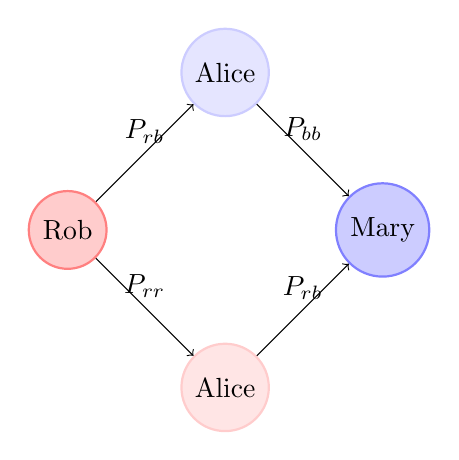
\begin{tikzpicture}
	\node at (0,0) [circle, draw=red!50, fill=red!20, thick] (r) {Rob};
	\node at (2,2) [circle, draw=blue!20, fill=blue!10, thick] (b) {Alice};
	\node at (4,0) [circle, draw=blue!50, fill=blue!20, thick] (g) {Mary};
	\node at (2,-2) [circle, draw=red!20, fill=red!10, thick] (br) {Alice};

	\draw [->] (r) -- (b) node[midway, above] {$P_{rb}$};
	\draw [->] (r) -- (br) node[midway, above] {$P_{rr}$};
	\draw [->] (b) -- (g) node[midway, above] {$P_{bb}$};
	\draw [->] (br) -- (g) node[midway, above] {$P_{rb}$};
\end{tikzpicture}
\end{center}	
I have called the unsampled case Alice but in reality we would know nothing about them apart from the fact that we must assume that they belong to one of the groups that we are looking at. For a given value of $\kappa$ we have to consider $2^\kappa$ different potential group combinations so for cases where $\kappa$ is large we will have to perform a lot of computations. Below is an example for when $\kappa = 2$ by adding Fred to the transmission path.
\begin{center}
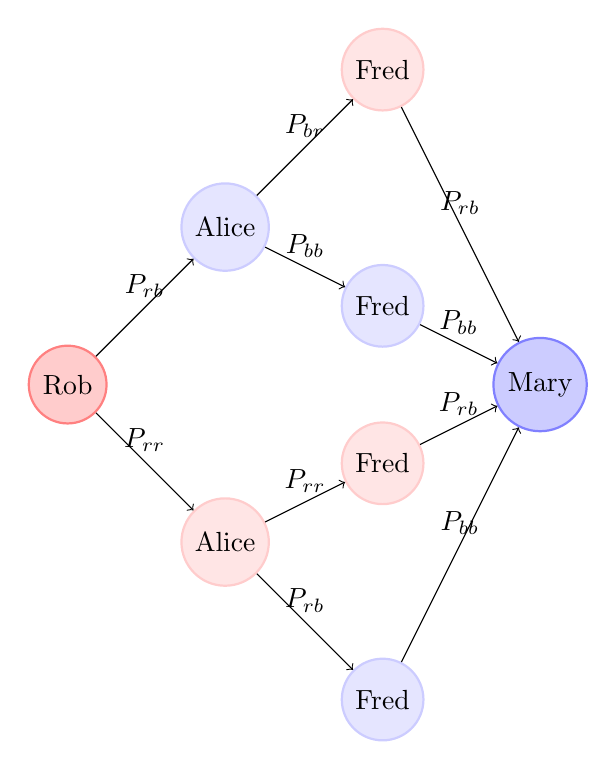
\begin{tikzpicture}
	\node at (0,0) [circle, draw=red!50, fill=red!20, thick] (r) {Rob};
	\node at (2,2) [circle, draw=blue!20, fill=blue!10, thick] (b) {Alice};
	\node at (6,0) [circle, draw=blue!50, fill=blue!20, thick] (g) {Mary};
	\node at (2,-2) [circle, draw=red!20, fill=red!10, thick] (br) {Alice};
	\node at (4,4) [circle, draw=red!20, fill=red!10, thick] (b2) {Fred};
	\node at (4,1) [circle, draw=blue!20, fill=blue!10, thick] (b3) {Fred};
	\node at (4,-1) [circle, draw=red!20, fill=red!10, thick] (br2) {Fred};
	\node at (4,-4) [circle, draw=blue!20, fill=blue!10, thick] (br3) {Fred};







	\draw [->] (r) -- (b) node[midway, above] {$P_{rb}$};
	\draw [->] (r) -- (br) node[midway, above] {$P_{rr}$};
	\draw [->] (b) -- (b2) node[midway, above] {$P_{br}$};
	\draw [->] (br) -- (br2) node[midway, above] {$P_{rr}$};
	\draw [->] (b) -- (b3) node[midway, above] {$P_{bb}$};
	\draw [->] (br) -- (br3) node[midway, above] {$P_{rb}$};
	\draw [->] (b2) -- (g) node[midway, above] {$P_{rb}$};
	\draw [->] (br2) -- (g) node[midway, above] {$P_{rb}$};
	\draw [->] (b3) -- (g) node[midway, above] {$P_{bb}$};
	\draw [->] (br3) -- (g) node[midway, above] {$P_{bb}$};



\end{tikzpicture}
\end{center}
If we have $n$ groups then calculating the group likelihood for a transmission event with $\kappa$ unsampled cases between them will require $n^\kappa$ individual calculations for each possible permutation of the different groups that the unsampled cases might belong to.



Kappa >1
Cartesian co-ordinates
\citet{outbrkr}
\bibliographystyle{plainnat}
\bibliography{references}

\end{document}